\section{System Sequence}
 \label{section:sequence}
 
To better visualize the interaction between components of the systems as well as its concrete functionalities, sequence diagrams for specific use cases are created. Each specific use cases are represented in a single sequence diagram, making it easier to convert the use case into corresponding technical user stories.

\subsection{Customer Validation on a Registration Event}
 \label{subsection:regis}

\begin{figure}[!ht]
 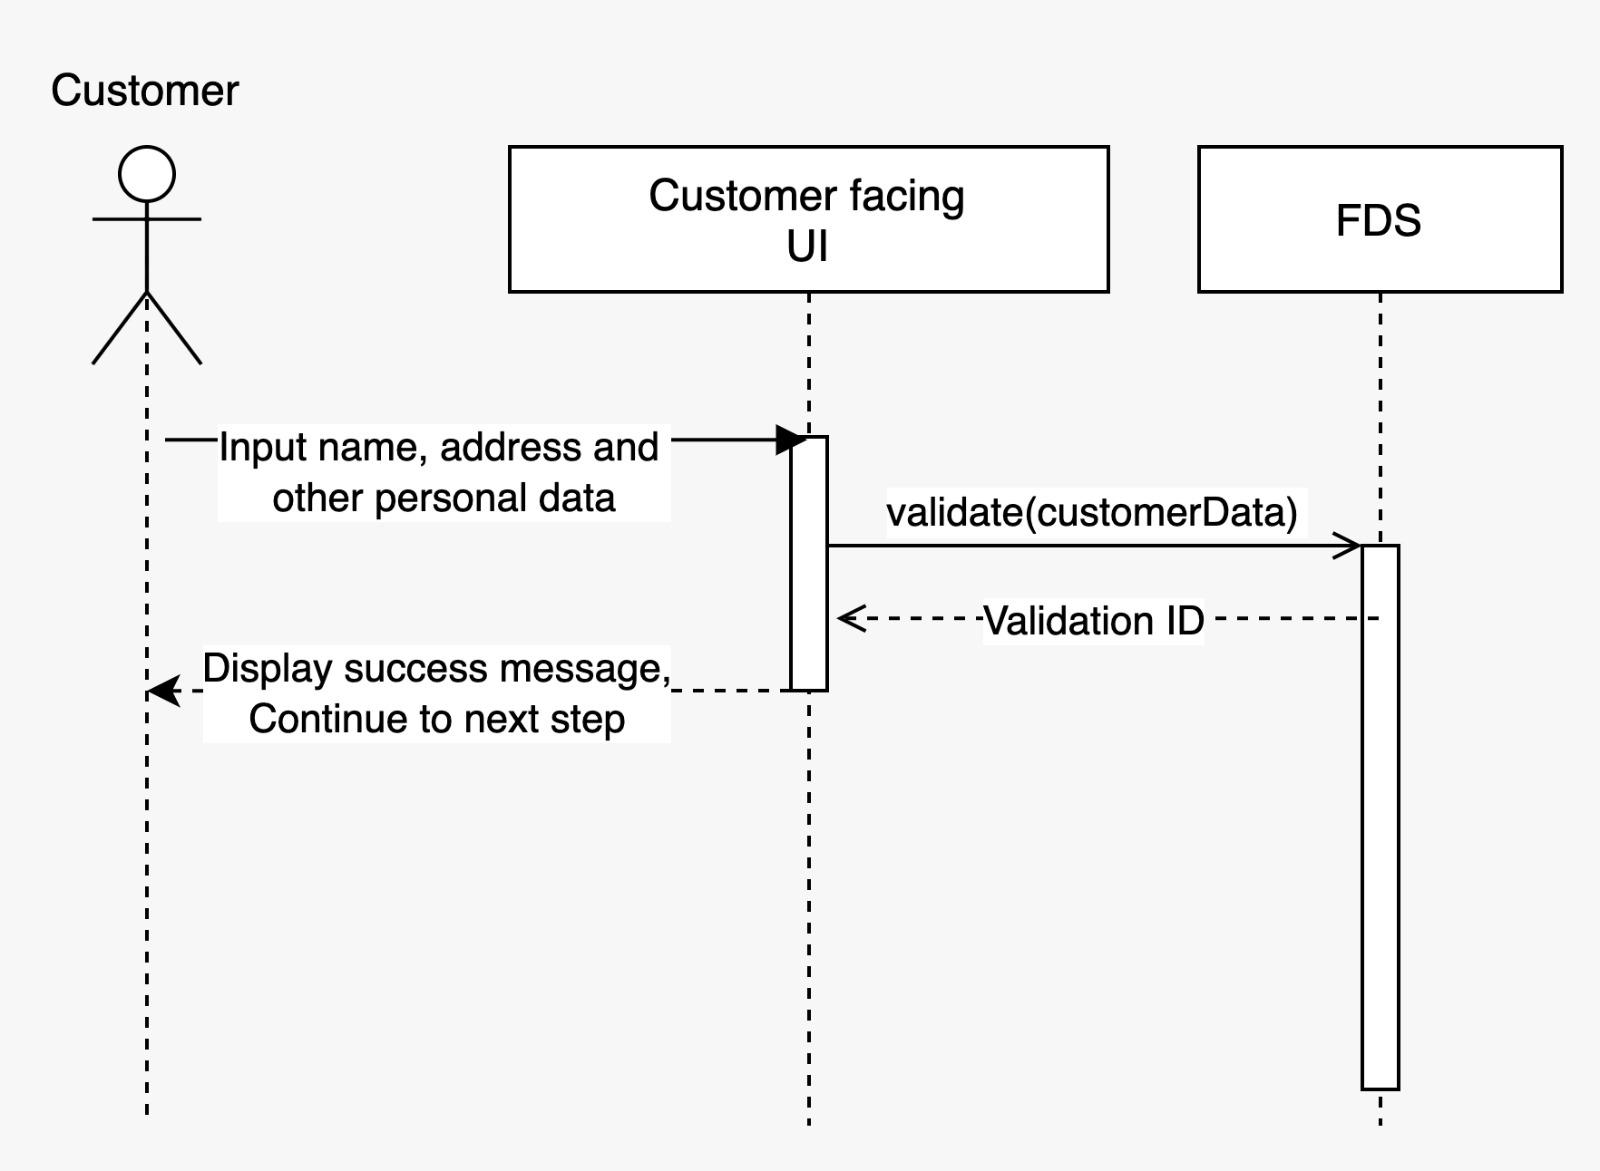
\includegraphics[width=\textwidth]{diagrams/sequence_registration.jpeg}
 \caption{System sequence diagram for a customer validation when a new customer is registered}
\end{figure}

A system sequence can be defined by analyzing the following use case:

\begin{quotation}
 \enquote{As a stakeholder, I want to verify users, so that the company can have more confidence that the existing user base is trustworthy} 
\end{quotation}

By further analysis of the use case listed above, the following sequence will be executed by the system:
\begin{itemize}
 \item A new customer inputs his or her personal data to a customer facing UI and clicks the \emph{"Register"} button
 \item The customer facing UI makes an HTTP Post request to the FDS, containing the user's personal data on its request payload
 \item The FDS receives the HTTP request, and schedules a new validation process to be executed asynchronously
 \item The FDS responds to the HTTP request by returning a validation ID pointing to the scheduled validation process
 \item Customer facing UI shows a success message and continues registration to the next step while the validation process runs 
\end{itemize}

\subsection{Notification on Suspicious Cases}
 \label{subsection:seq-notification}

\begin{figure}[!h]
 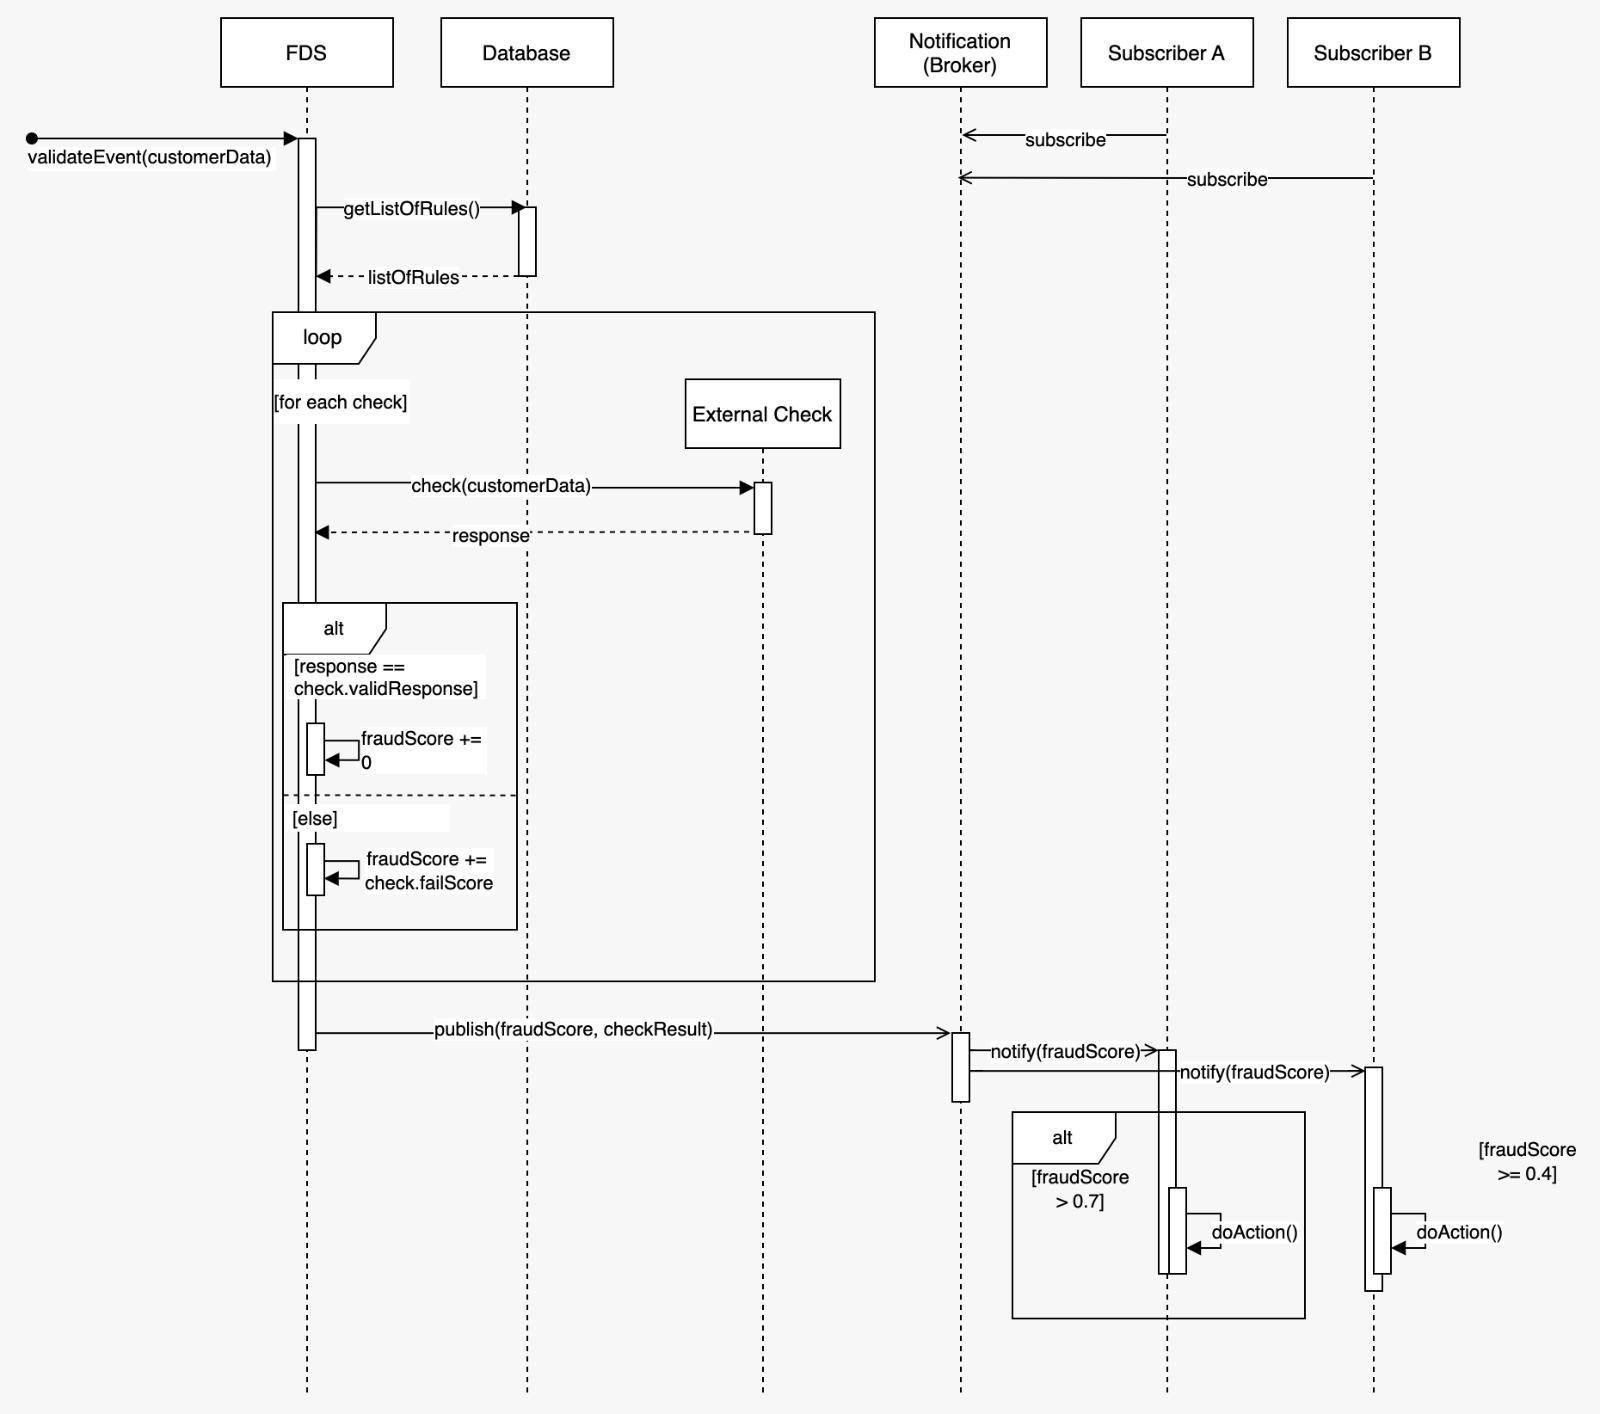
\includegraphics[width=\textwidth]{diagrams/sequence_notification.jpeg}
 \caption{System sequence diagram for notifications on suspicious cases}
\end{figure}

To fulfill the requirements listed on \textbf{TODO: Link Analysis}, a further examination of the following use case should be done:

\begin{quotation}
 \enquote{As an employee, I want to be notified when a user seems suspicious, so that I can do necessary actions accordingly} 
\end{quotation}

As a result, the following sequence will be executed by the system:

\begin{itemize}
 \item The FDS receives an HTTP request to schedule a validation process and responds by returning the ID of the validation process
 \item FDS retrieves a list of validation rules from the database
 \item FDS begins to initiate a validation process by setting the fraud score to 0 and looping through the list of validation rules for evaluation
 \item A validation rule will be evaluated by making an HTTP request to the external endpoint defined by the validation rule and evaluating its response according to the condition specified
 \item If the response matches all the conditions specified by the validation rule, the rule evaluation will be considered as a success and the fraud score will be incremented with 0. Otherwise, the rule evaluation will be considered as a failure and the fraud score will be incremented by the \emph{fail score} specified by the validation rule
 \item After the evaluation of all validation rules retrieved from the database is completed, the FDS publishes the validation result to an exchange hosted created the message broker
 \item The message consumers consume the message from the exchange and react accordingly\footnote{For example: sending an email notification if the fraud score exceeds 0.7.}
\end{itemize}

\subsection{Managing Validation Rules}
 \label{subsection:management}

\begin{figure}[!ht]
 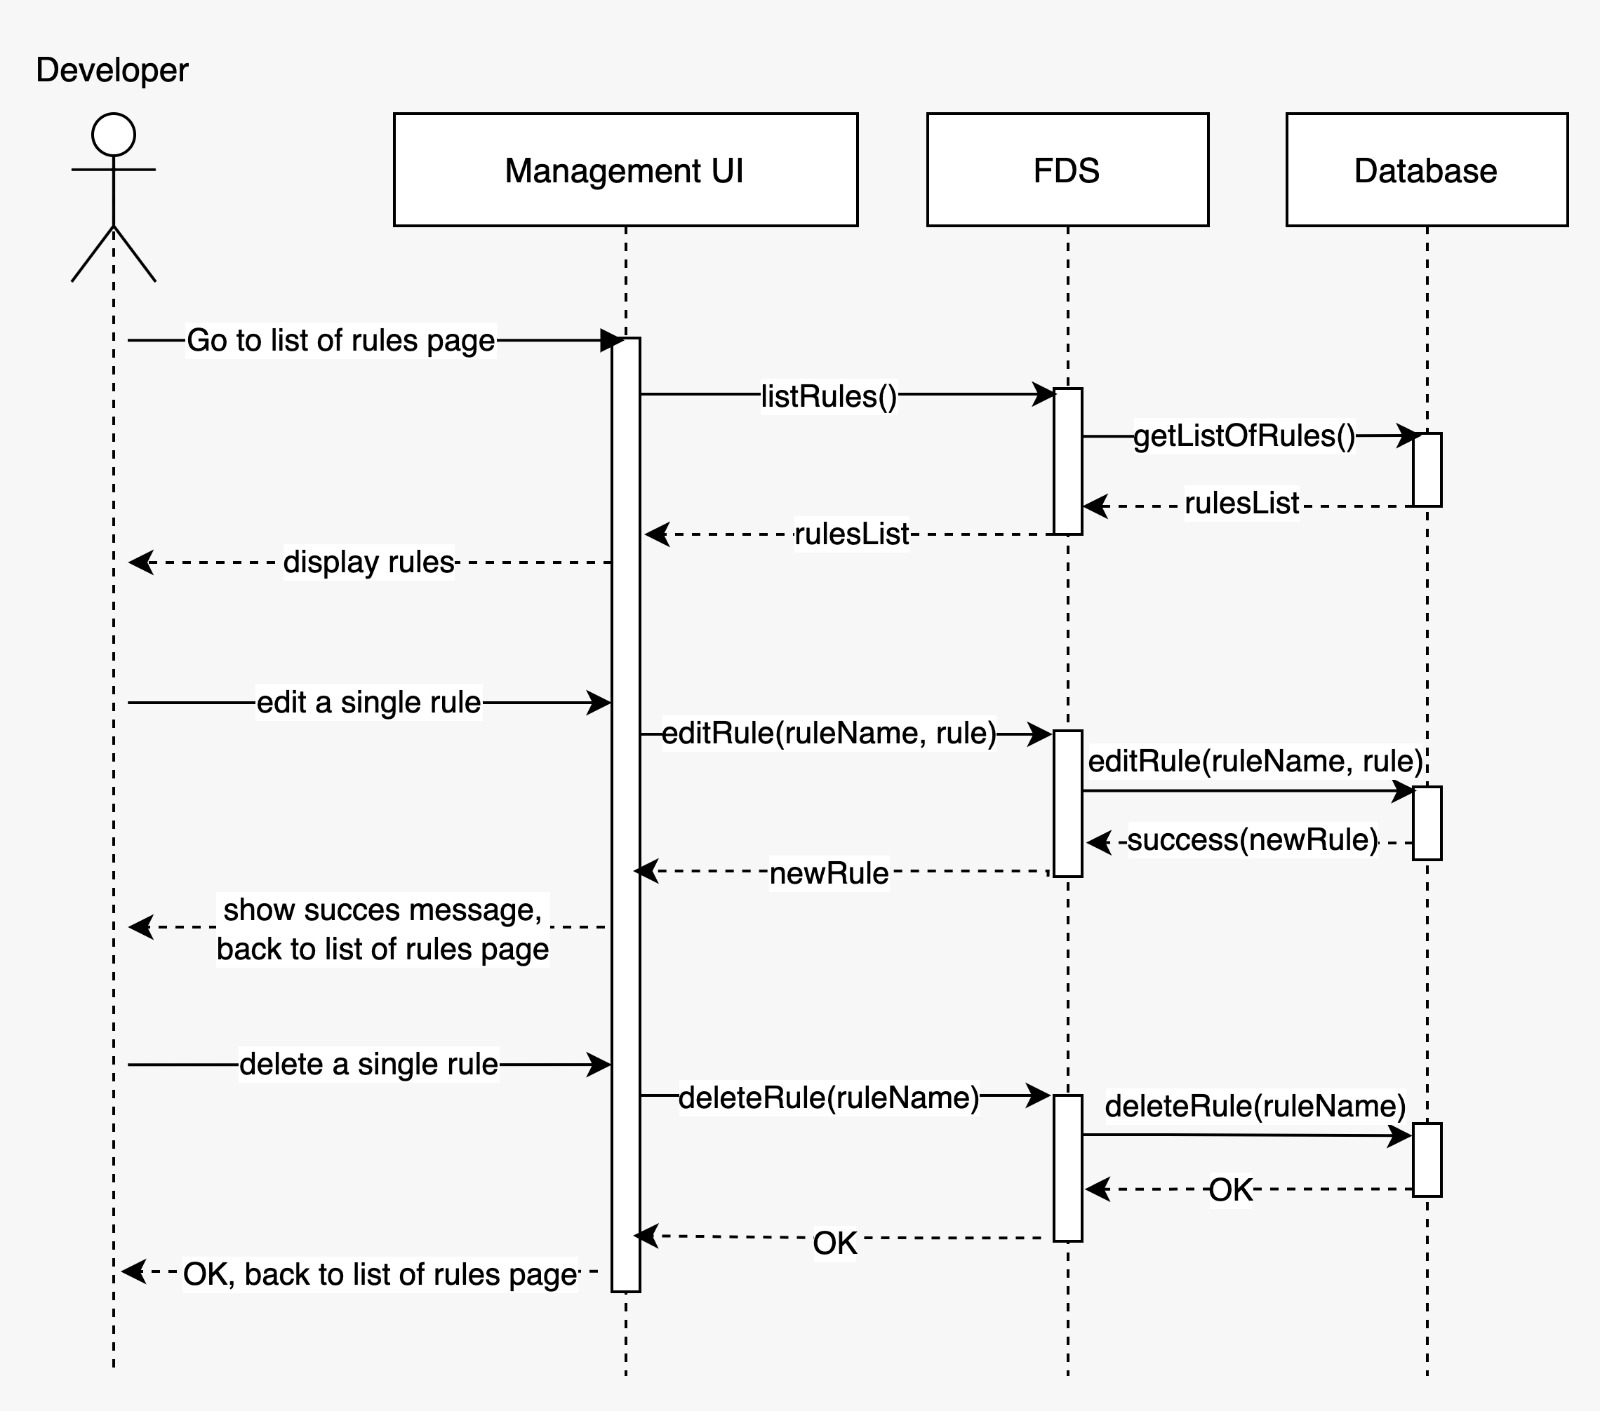
\includegraphics[width=\textwidth]{diagrams/sequence_management.jpeg}
 \caption{System sequence diagram for validation rules management}
\end{figure}


Another sequence can also be defined as a result of an analysis of the following use case:

\begin{quotation}
 \enquote{As an employee, I want to manage my own rule to validate users, so that I can use my expertise to find suspicious customers as efficiently as possible without the communication overhead with other teams} 
\end{quotation}

The following sequence will be executed by the system as a detailed flow for a validation rule management:

\begin{itemize}
 \item A user (e.g. Developer) can access the management UI and go to the page that displays a list of available validation rules
 \item The FDS retrieves a list of validation rules from the database
 \item User can click on a single rule and edit the rule
 \item The management UI makes an HTTP PUT\footnote{In \autocite[\enquote{9.6 PUT}]{http-rfc}, HTTP PUT method is described as a method to store or modify an entity, defined by the Request-URI.} request to the database to edit an existing rule
 \item The FDS receives the HTTP request, modify the rule on the database and returns the edited rule as a response
 \item The management UI displays a success message and redirects user back to the list of rules page
 \item User can click on a single rule and delete the rule
 \item The management UI makes an HTTP DELETE\footnote{In \autocite[\enquote{9.7 DELETE}]{http-rfc}, HTTP DELETE method is described as a method to delete a resource on the host server, pointed by the Request-URI.} request to the database to delete an existing rule
 \item The FDS receives the HTTP request and delete the rule on the database, returning a 204\footnote{In \autocite[\enquote{10.2.5 204 No Content}]{http-rfc}, the 204 status code should be used if the server fulfilled the request, but no data should be returned by the HTTP response.} status code as an identifier of a successful operation
 \item The management UI displays a success message and redirects user back to the list of rules page
\end{itemize} 